% vim: set textwidth=78 autoindent:

%\subsection{Interpolation Plugin}
%
%% when the revision of a section has been finalized, 
%% comment out the following line:
%%\updatedisclaimer
%
%The Interplation plugin allows to interpolate a TIN or IDW raster layer from a vector 
%point layer loaded in the QGIS canvas. It is very simple to handle and provides 
%functionalities as shown in Figure \ref{fig:interpolation_dialog}.

\subsection{Extension d'interpolation}

Cette extension permet d'interpoler une couche raster TIN ou IDW depuis une couche vecteur de points, elle est très facile à utiliser comme le montre la figure \ref{fig:interpolation_dialog}.

%\begin{itemize}
%\item \textbf{Input vector layer}: Select vector point layer loaded in the QGIS canvas.
%\item \textbf{Interpolation attribute}: Select attribute column used for interpolation or 
%enable \checkbox{Use Z-Coordinate} checkbox.
%\item \textbf{Interpolation Method}: Select interpolation method \selectstring{Triangulated Irregular 
%Network (TIN)}{\ldots} or \selectstring{Inverse Distance Weighted (IDW)}{\ldots}.
%\item \textbf{Number of columns/rows}: define number colums and.rows for the output raster file
%\item \textbf{Output file}: Define a name for the output raster file
%\end{itemize}

\begin{itemize}
\item \textbf{Couche vectorielle de saisie}: Sélectionnez une couche vectorielle de points présente dans la fenêtre carte de QGIS.
\item \textbf{Interpolation attribute}: Sélectionnez la colonne attributaire utilisée pour l'interpolation, ou 
cochez la case \checkbox{Utilisez les coordonnées Z pour l'interpolation}.
\item \textbf{Méthode d'interpolation}: Sélectionnez une méthode d'interpolation : \selectstring{Interpolation Triangulaire (TIN)}{\ldots} ou\selectstring{Pondération par Distance Inverse (IDW)}{\ldots}.
\item \textbf{Nombre de colonnes/lignes}: Définit le nombre de lignes et de colonnes du raster de sortie.
\item \textbf{Fichier de sortie}: Définit un nom pour le fichier raster de sortie.
\end{itemize}

%\begin{figure}[ht]
%   \begin{center}
%   \caption{Interpolation Plugin \nixcaption}\label{fig:interpolation_dialog}\smallskip
%   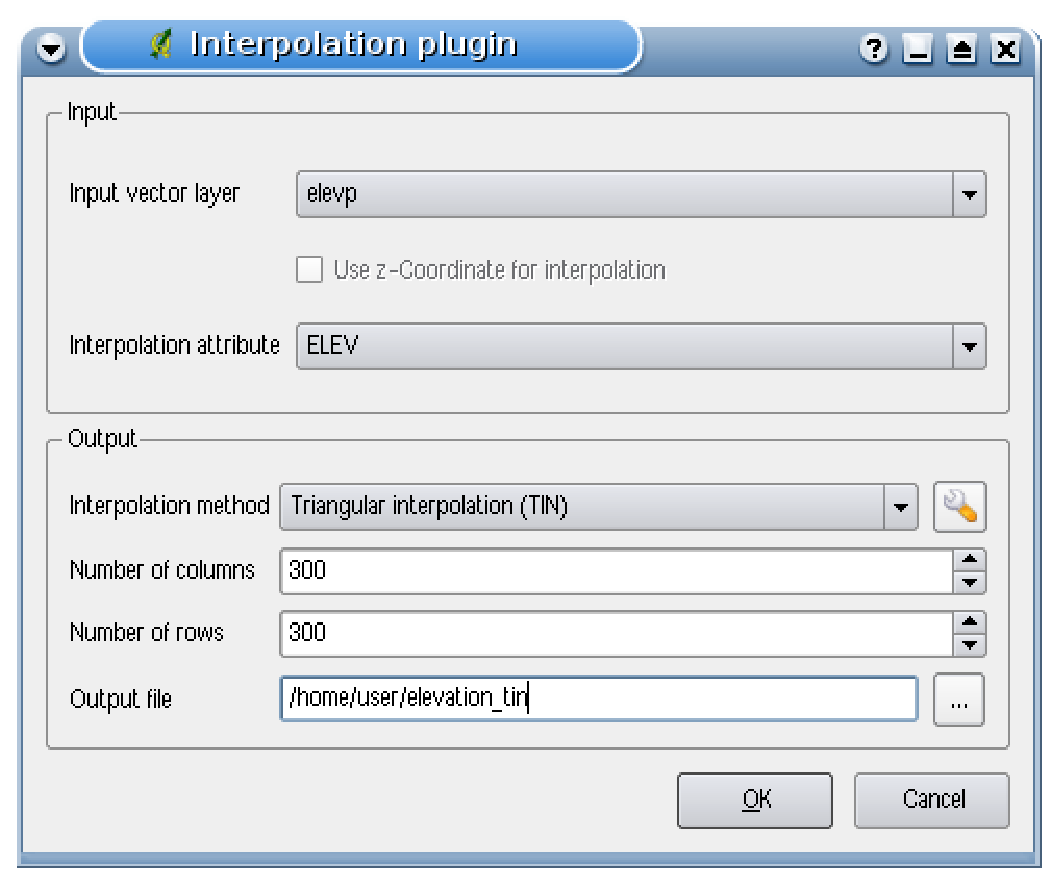
\includegraphics[clip=true, width=9cm]{interpolate_dialog}
%\end{center}  
%\end{figure}

\begin{figure}[ht]
   \begin{center}
   \caption{Interpolation Plugin \nixcaption}\label{fig:interpolation_dialog}\smallskip
   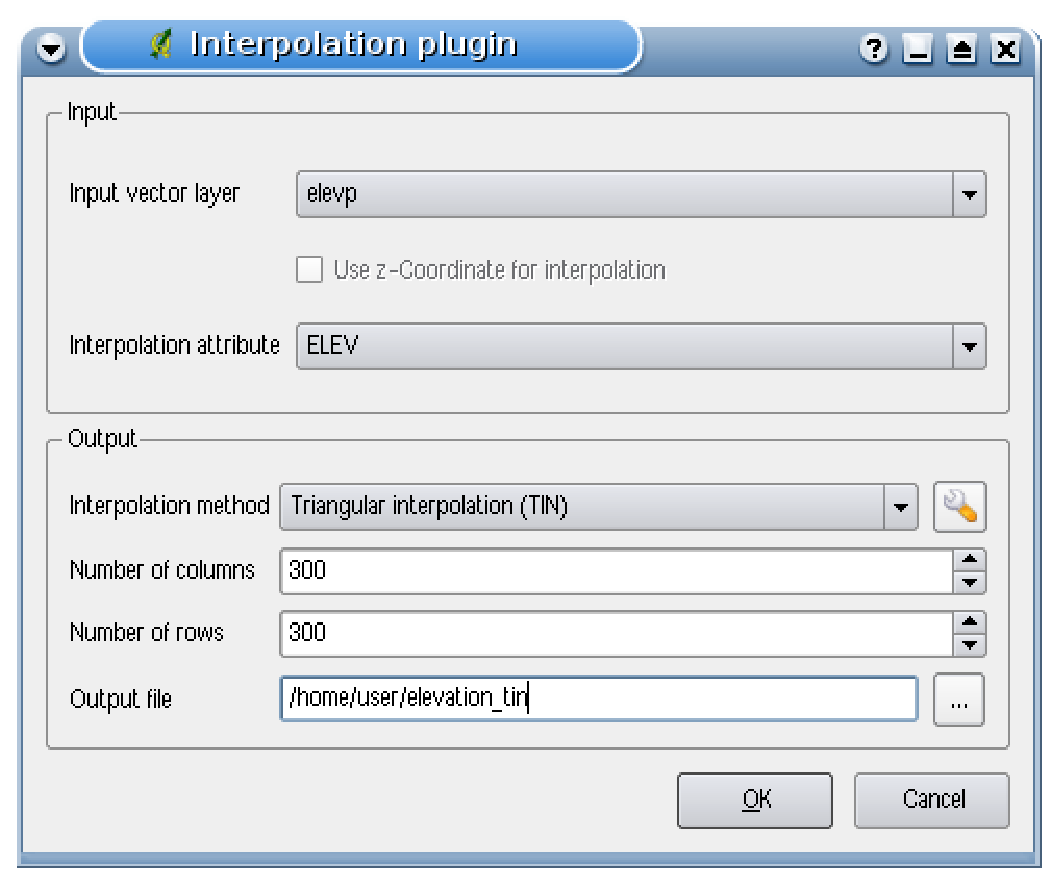
\includegraphics[clip=true, width=9cm]{interpolate_dialog}
\end{center}  
\end{figure}

%\begin{enumerate}
%  \item Start QGIS and load the \filename{elevp.csv} CSV table with elevation points in the QGIS 
%  canvas using the delimited text plugin as described in Section \ref{label_dltext}. 
%  \item Load the Interpolation plugin in the Plugin Manager (see Section 
%  \ref{sec:load_core_plugin}) and click on the \toolbtntwo{interpolation}{Interpolation} 
%  icon which appears in the QGIS toolbar menu. The Interpolation plugin dialog appears as shown in Figure \ref{fig:interpolation_dialog}.
%  \item Select \selectstring{elevp}{\ldots} as input vector and column \filename{ELEV} for 
%  interpolation.
%  \item Select \selectstring{Triangular interpolation}{\ldots} as interpolation method, define 
%  3663 cols and 1964 rows (this is equivalent to a 1000 meter pixel resolution) as raster 
%  output filename \filename{elevation\_tin}.
%  \item Click \button{Ok}.
%  \item Double click \filename{elevation\_tin} in the map legend to open the Raster Layer Properties 
%  dialog and select \selectstring{Pseudocolor}{\ldots} as Color Map in the \tab{Symbology} tab. Or you 
%  can define a new color table as described in Section \ref{label_rasterprop}.
%\end{enumerate}

\begin{enumerate}
  \item Lancez QGIS et chargez le tableau CSV \filename{elevp.csv} contenant les points d'élévations dans le canevas de QGIS en utilisant l'extension décrite dans la section \ref{label_dltext}. 
  \item Chargez l'extension d'Interpolation (voir la section \ref{sec:load_core_plugin}) et cliquez sur le bouton \toolbtntwo{interpolation}{Interpolation} qui apparaît dans le menu de la barre d'outils. Un nouveau dialogue se présente comme l'illustre la figure \ref{fig:interpolation_dialog}.
  \item Sélectionnez \selectstring{elevp}{\ldots} comme entrée de vecteur et la colonne \filename{ELEV} pour l'interpolation.
  \item Sélectionnez \selectstring{Interpolation Triangulaire}{\ldots} comme méthode d'interpolation, définissez 3663 colonnes et 1964 lignes (ce qui équivaut à une résolution par pixel de 1000 mètres) et \filename{elevation\_tin} comme nom pour le fichier en sortie.
  \item Cliquez sur \button{Ok}.
  \item Double-cliquez sur \filename{elevation\_tin} dans la légende de la carte pour ouvrir la fenêtre de propriétés de la couche raster et sélectionnez \selectstring{Pseudocouleur}{\ldots} comme couleurs pour la carte dans l'onglet \tab{Symbologie}. Vous pouvez aussi définir une nouvelle table de couleurs comme expliquée dans la section \ref{label_rasterprop}.
\end{enumerate}

%In Figure \ref{fig:interpolation_idw} you see the IDW interpolation result with a 366 cols x 196 rows (10 km) 
%resolution for the \filename{elevp.csv} data visualized using the Pseudocolor color table. The processing 
%takes a couple of minutes, although the data only cover the northern part of Alaska.
%
%\begin{figure}[ht]
%   \begin{center}
%   \caption{Interpolation of elevp data using IDW method \nixcaption}\label{fig:interpolation_idw}\smallskip
%   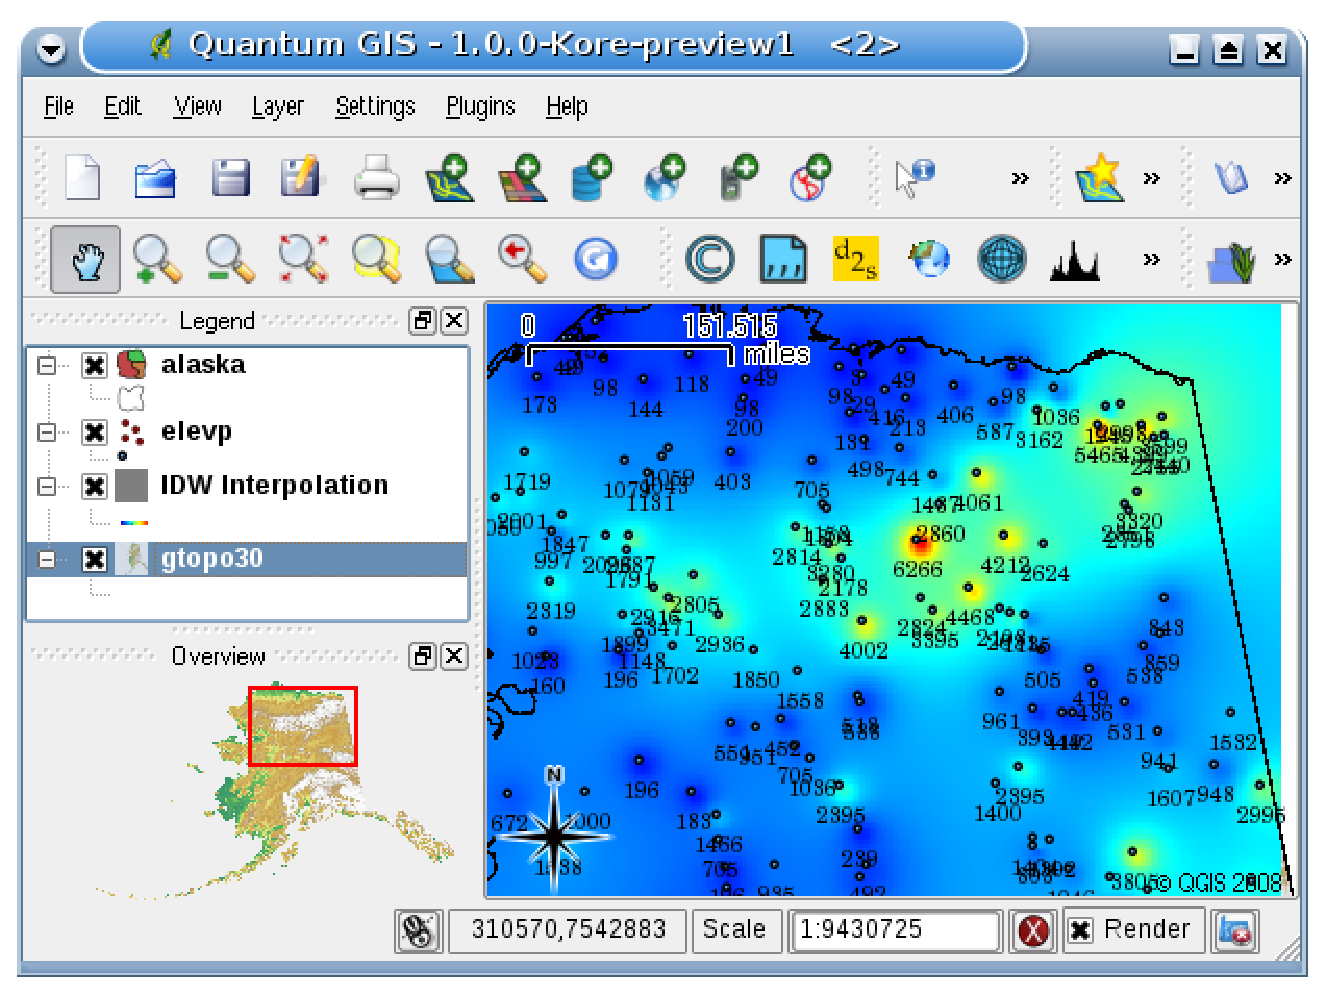
\includegraphics[clip=true, width=\textwidth]{interpolate_idw}
%\end{center}  
%\end{figure}
%
%\newpage

Dans la figure \ref{fig:interpolation_idw} vous pouvez voir le résultat d'une interpolation IDW avec une résolution de 366 colonnes x 196 lignes (soit 10 km), pour les données du fichier \filename{elevp.csv}. Le calcul peut prendre plusieurs minutes même si les données ne couvrent que la partie nord de l'Alaska.

\begin{figure}[ht]
   \begin{center}
   \caption{Interpolation d'une carte d'élévation en utilisant la méthode IDW \nixcaption}\label{fig:interpolation_idw}\smallskip
   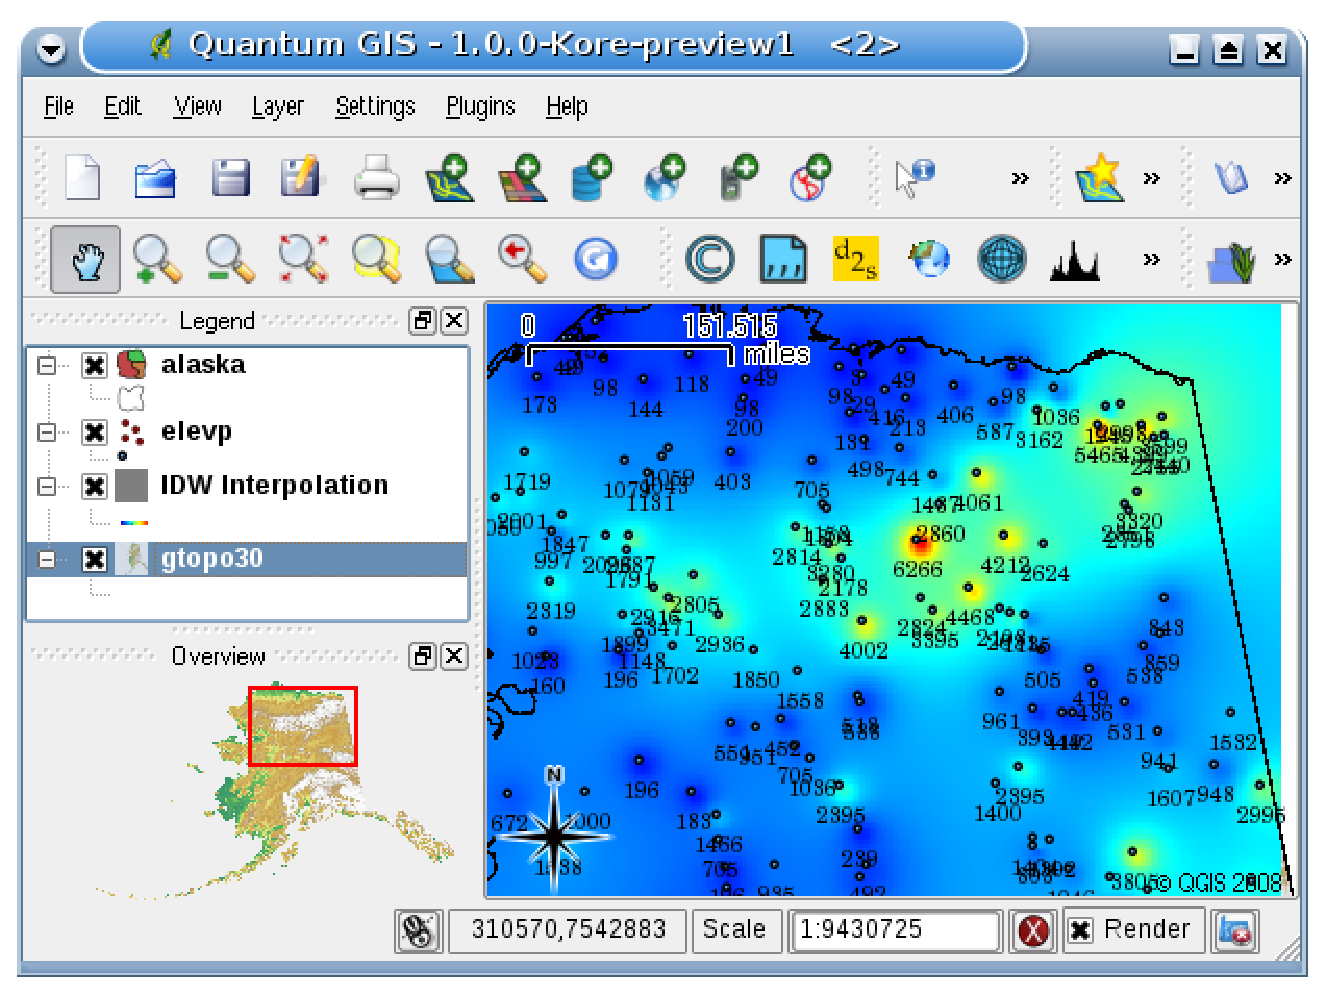
\includegraphics[clip=true, width=\textwidth]{interpolate_idw}
\end{center}  
\end{figure}

\newpage